\chapter{Theoretical background}\label{background}

In this chapter, we intend to provide the necessary background to the user
to understand the mechanisms used later in the work. The description of
each system is only a short introduction to familiarize the reader with
the needed concepts.

Specifically, section \ref{sec:gzip} describes the functionality of the gzip
compression software and the algorithms that it entails. Section
\ref{sec:sameorigin} covers the same-origin policy that applies in the web
application security model. In section \ref{sec:tls} we explain Transport
Layer Security, which is the widely used protocol that provides communications
security over the Internet. Finally, in section \ref{sec:mitm} we describe
attack methodologies, such as ARP spoofing, in order for an
adversary to perform a Man-in-the-Middle attack.

\section{gzip}\label{sec:gzip}

gzip is a file format and a software application used for file compression and
decompression. It is the most popular compression method on the Internet, integrated
into protocols such as HTTP and XMPP. Derivatives of gzip include the tar utility, which 
can extract .tar.gz files, as well as zlib, an abstraction of the DEFLATE algorithm in 
library form.\footnote{\url{https://en.wikipedia.org/wiki/Gzip}}

It is based on the DEFLATE algorithm, which is a composition of LZ77 and Huffman
coding. DEFLATE could be described in short by the following compression schema:

\begin{math}DEFLATE(m) = Huffman(LZ77(m))\end{math}

In the following sections we will briefly describe the functionality of both
these compression algorithms.

\subsection{LZ77}\label{subsec:lz77}

LZ77 is a lossless data compression algorithm published by A. Lempel and J. Ziv
in 1977 \cite{lz77}. It achieves compression by replacing repeated occurrences 
of data with references to a single copy of that data existing earlier in the 
uncompressed data stream. A match is encoded by a pair of numbers called a 
length-distance pair, the first of which represents the length of the repeated
portion and the second of which describes the distance backwards in the stream.
In order to spot repeats, the protocol needs to keep track of some amount of the
most recent data, specifically the latest 32 kilobytes. This data is held in a
sliding window, therefore the initial appearance of a portion of data needs to have occurred
at most 32 Kb up the data stream, in order to be compressed. Also, the minimum
length of a text that can be compressed is 3 characters. Compressed text can
refer to literals as well as pointers.

Below you can see an example of a step-by-step execution of the algorithm for a
chosen text:

\begin{figure}[H] \caption{Step 1: Plaintext to be compressed} \centering
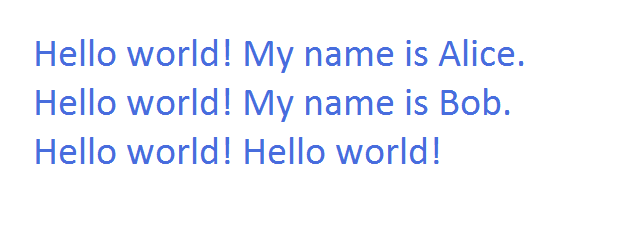
\includegraphics[width=0.5\textwidth]{diagrams/lz77_1.png}\end{figure}
\begin{figure}[H] \caption{Step 2: Compression starts with literal
representation} \centering
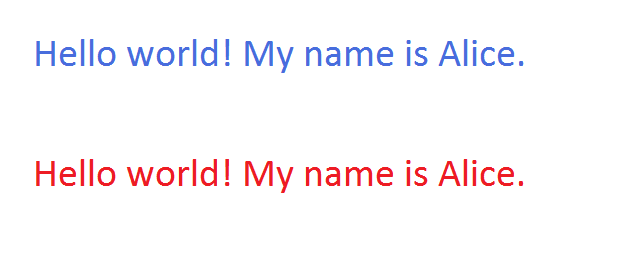
\includegraphics[width=0.35\textwidth]{diagrams/lz77_2.png}\end{figure}
\begin{figure}[H] \caption{Step 3: Use a pointer at distance 31 and length 25}
\centering
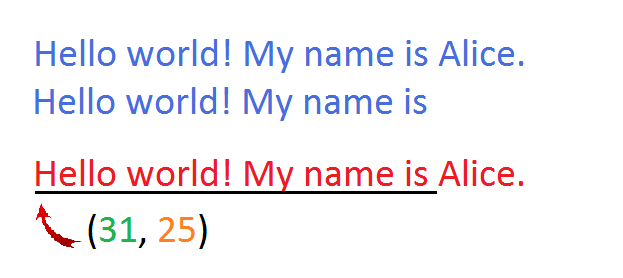
\includegraphics[width=0.35\textwidth]{diagrams/lz77_3.png}\end{figure}
\begin{figure}[H] \caption{Step 4: Continue with literal} \centering
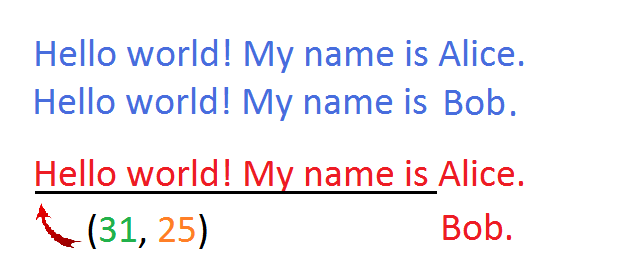
\includegraphics[width=0.35\textwidth]{diagrams/lz77_4.png}\end{figure}
\begin{figure}[H] \caption{Step 5: Use a pointer pointing to a pointer}
\centering
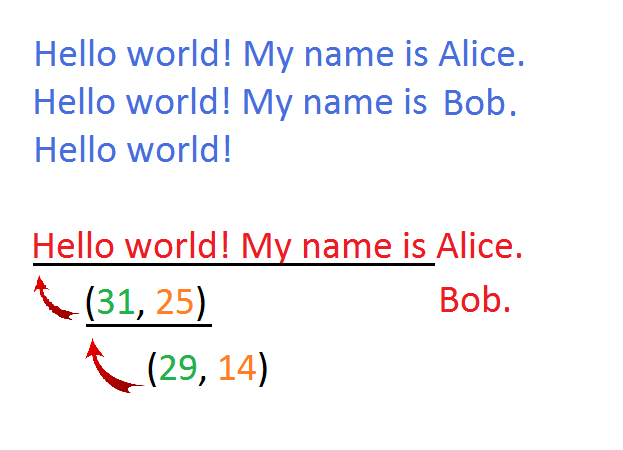
\includegraphics[width=0.35\textwidth]{diagrams/lz77_5.png}\end{figure}
\begin{figure}[H] \caption{Step 6: Use a pointer pointing to a pointer pointing
to a pointer} \centering
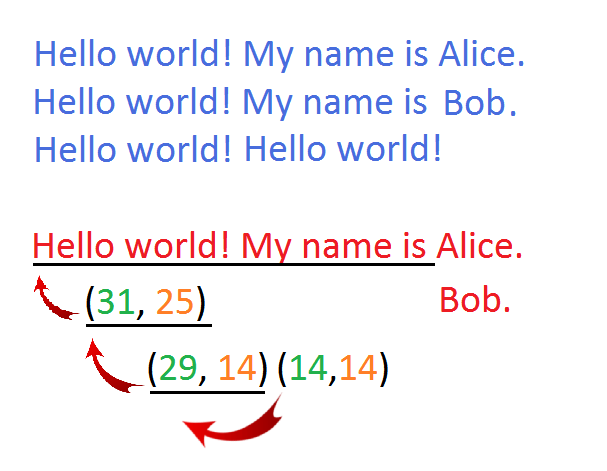
\includegraphics[width=0.35\textwidth]{diagrams/lz77_6.png}\end{figure}


\subsection{Huffman coding}\label{subsec:huffman}

Huffman coding is also a lossless data compression algorithm developed by David
A. Huffman and published in 1952 \cite{huffman}. When compressing a text with
this algorithm, a variable-length code table is created to map source symbols to
bit streams. Each source symbol can be represented with less or more bits
compared to the uncompressed stream, so the mapping table is used to translate
source symbols into bit streams during compression and vice versa during
decompression. The mapping table could be represented as a binary tree of nodes,
where each leaf node represents a source symbol, which can be accessed from the 
root of the tree by following the left path for 0 and the right path for 1. Each
source symbol can be represented only by leaf nodes, therefore the code is
prefix-free, i.e. no bit stream representing a source symbol can be the prefix
of any other bit stream representing a different source symbol. The final
mapping of source symbols to bit streams is calculated by finding the frequency
of appearance of each source symbol of the plaintext. That way, most common
symbols will be coded in shorter bit streams, resulting in a compression of the 
initial text. Finally, the compression mapping needs to be included in the final
compressed text so that it can be used during decompression.

Below follows an example of a plaintext and a valid Huffman tree that can be
used for compressing it:

\bigskip \centerline{\textit{\textbf{Would a helium balloon float on the moon?}}}

\bigskip \centerline{\textbf{Frequency Analysis}}

\begin{table}[H] \centering \begin{tabular}{ | l | l | l | l | } \hline
\textbf{o}: 7 & \textbf{l}: 5 & \textbf{a}: 3 & \textbf{n}: 3 \\ \textbf{u}: 2 &
\textbf{h}: 2 & \textbf{e}: 2 & \textbf{m}: 2 \\ \textbf{t}: 2 & \textbf{w}: 1 &
\textbf{d}: 1 & \textbf{i}: 1 \\ \textbf{b}: 1 & \textbf{f}: 1 & \textbf{}  & \textbf{}
\\ \hline \end{tabular} \end{table}

\centerline{\textbf{Huffman tree}}

\begin{table}[H] \centering \begin{tabular}{ | l | l | l | l | } \hline
\textbf{o}: 00 & \textbf{l}: 01 & \textbf{a}: 1000 & \textbf{n}: 1001 \\
\textbf{u}: 1010 & \textbf{h}: 1011 & \textbf{e}: 11000 & \textbf{m}: 11001 \\
\textbf{t}: 11010 & \textbf{w}: 11011 & \textbf{d}: 11100 & \textbf{i}: 1111000
\\ \textbf{b}: 1111001 & \textbf{f}: 1111010 & \textbf{}  & \textbf{}
\\ \hline \end{tabular} \end{table}

\centerline{\textbf{Initial text size: 264 bits}} \centerline{\textbf{Compressed
text size: 133 bits}}


\section{Same-origin policy}\label{sec:sameorigin}

Same-origin policy is an important aspect of the web application security model. 
Under the policy, a web browser permits scripts contained in a first web page 
to access data in a second web page, but only if both web pages have the same 
origin. An origin is defined as a combination of Uniform Resource Identifier scheme
\footnote{\url{https://en.wikipedia.org/wiki/Uniform_resource_identifier}}, hostname,
and port number. This policy prevents a malicious script on one page from obtaining
access to sensitive  data on another web page through that page's Document Object
Model\footnote{\url{https://en.wikipedia.org/wiki/Document_Object_Model}}.

The following table explains same-origin-policy. We assume that we want access from \\
http://www.test.com/dir/test.html to each of the following URLs:


\begin{table}[H] \centering \begin{tabular}{ | l | l | l | } \hline
\textbf{Compared URL} & \textbf{Result} & \textbf{Reason}   \\
http://www.test.com/dir/page.html & Success & Same protocol/host \\
http://www.test.com/dir2/other.html & Success & Same protocol/host \\
http://www.test.com:81/dir2/other.html & Failure & Same protocol/host, different port \\
https://www.test.com/dir2/other.html & Failure & Different protocol \\
http://www.en.test.com/dir2/other.html & Failure & Different host \\
\hline \end{tabular} \end{table}


This mechanism is particularly significant for modern web applications that extensively 
depend on HTTP cookies to maintain authenticated user sessions. The lack of same origin
policy would result in the compromise of data confidentiality or integrity. Despite the
use of same-origin policy by modern browsers, there still exist attacks that enable an
adversary to bypass it and compromise a user's communication with a website. Two major
types of such attacks, cross-site scripting (XSS) and cross-site request forgery (CSRF)
are described in the following subsections.

\subsection{Cross-site scripting}

Cross-Site Scripting (XSS) attacks are a type of injection, in which malicious scripts 
are injected into otherwise benign and trusted web sites. XSS attacks occur when an attacker 
uses a web application to send malicious code, generally in the form of a browser side
script, to a different end user. That way, same-origin policy can be bypassed and sensitive
data handled by the vulnerable website may be compromised.

XSS attacks can generally be categorized into two categories: \texttt{stored} and \texttt{reflected}.

\texttt{Stored XSS Attacks} are those where the injected script is permanently stored on
the target servers , such as in a database, in a message forum. The victim then retrieves
the malicious script from the server when it requests the stored information.

\texttt{Reflected XSS Attacks} are those where the injected script is reflected off the web
server, such as in an error message, search result, or any other response that includes some
or all of the input sent to the server as part of the request.

For further information on XSS refer to \cite{xssowasp}.

\subsection{Cross-site request forgery}

Cross-Site Request Forgery (CSRF) is an attack that forces an end user to execute unwanted
actions on a web application in which they are currently authenticated. CSRF attacks
specifically target state-changing requests, not theft of data, since the attacker has
no way to see the response to the forged request.
An attacker may trick the users of a web application into executing actions of the attacker's
choosing. If the victim is a normal user, a successful CSRF attack can force the user to perform
state changing requests like transferring funds, changing their email address, and so forth.
If the victim is an administrative account, CSRF can compromise the entire web application.

For example, when Alice visits a web page that contains the HTML image tag
\textit{<img src="\url{http://bank.example.com/withdraw?account=Alice&amount=1000000&for=Mallory}">},
that Mallory has injected, a request from Alice's browser to the
\texttt{example} bank's website will be issued, stating an amount of
1.000.000 to be transferred from Alice's account to Mallory's. If Alice is
logged in the \texttt{example} bank's website, the browser will include the
cookie containing Alice's authentication information in the request, validating
the request for the transfer. If the website does not perform more sanity checks
or further validation from Alice, the unauthorized transaction will be
completed. An attack like this is very common on Internet forums, where users
are allowed to post images.

\section{Transport Layer Security}\label{sec:tls}

Transport Layer Security (TLS) is a cryptographic protocol that provide communications
security over a computer network, allowing a server and a client to communicate in a way
that prevents eavesdropping, tampering or message forgery.

TLS is composed of two layers:
the TLS Record Protocol and the TLS Handshake Protocol. The Record Protocol 
provides connection security, while the Handshake Protocol allows the server 
and client to authenticate each other and negotiate encryption algorithms 
and cryptographic keys before any data is exchanged.

One category of TLS attack is compression attacks \cite{compression_attacks}. 
Such attacks exploit TLS-level compression in order to decrypt ciphertext. 
In this work, we extend the usability and optimize the performance of such an attack, 
BREACH\footnote{\url{http://breachattack.com}}


\subsection{TLS handshake}

\begin{figure}[H] \caption{TLS handshake flow} \centering
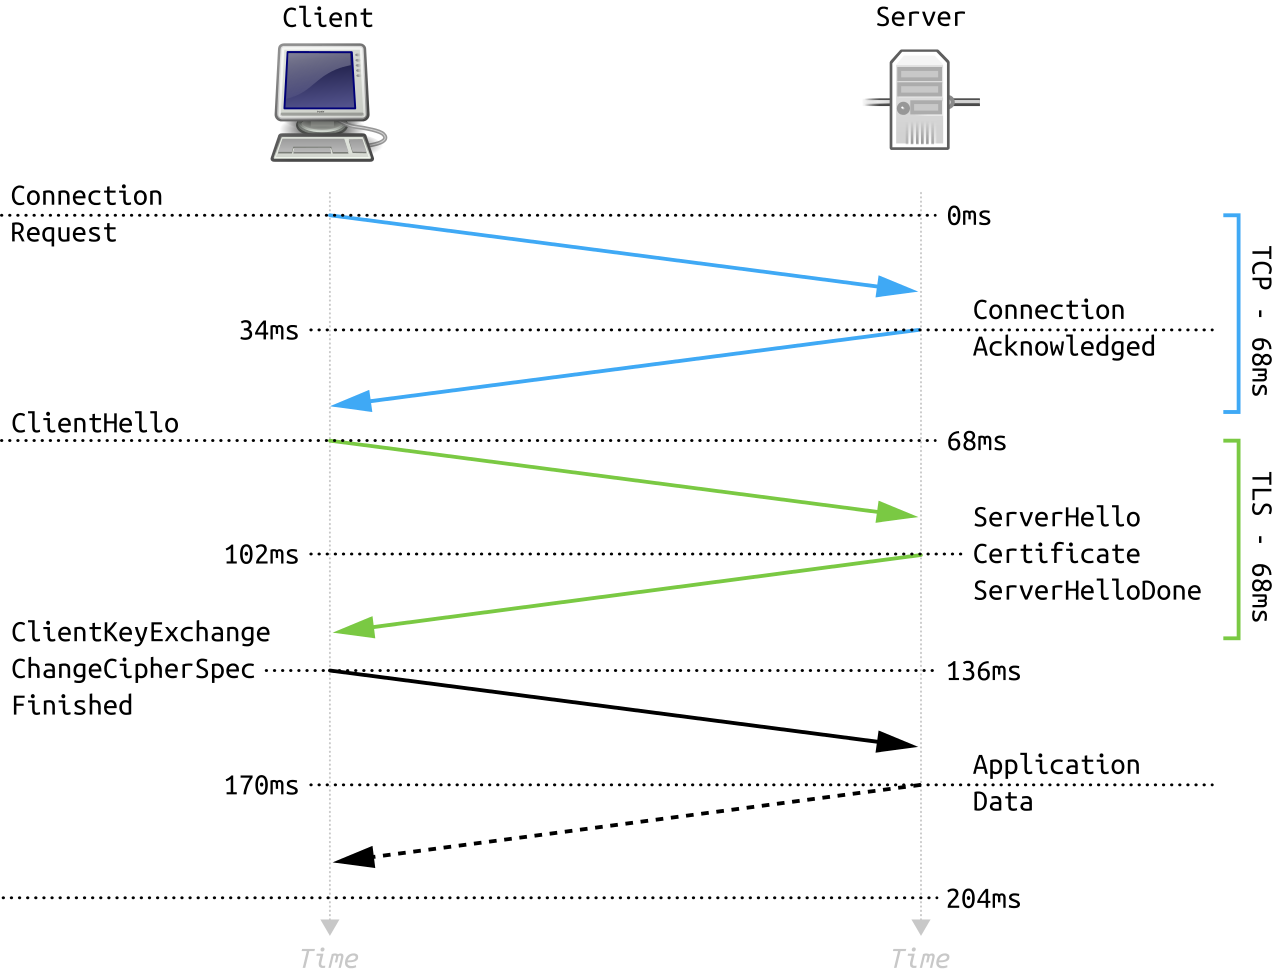
\includegraphics[width=0.7\textwidth]{diagrams/tls_handshake.png}\end{figure}

The above sequence diagram presents the functionality of a TLS handshake.
The client and the server exchange the basic parameters of the connection such as 
the highest TLS protocol version, a random number, a list of suggested cipher 
suites and suggested compression methods. The server provides the client with all
the necessary information in order to validate and use the asymmetric server key
to compute the symmetric key that will be used for the rest of the communication.
The client computes the  PreMasterSecret and sends it to the server 
which is then used by both parties to compute the symmetric key.
Finally, both sides exchange and validate hash and MAC codes over all the
previous messages, after which they both have the ability to communicate safely.

This applies only in the basic TLS handshake. Client-authenticated and resumed handshakes
are quite different, although they are not relevant for the purpose of this work.


\subsection{TLS record}

\begin{figure}[H] \caption{TLS record} \centering
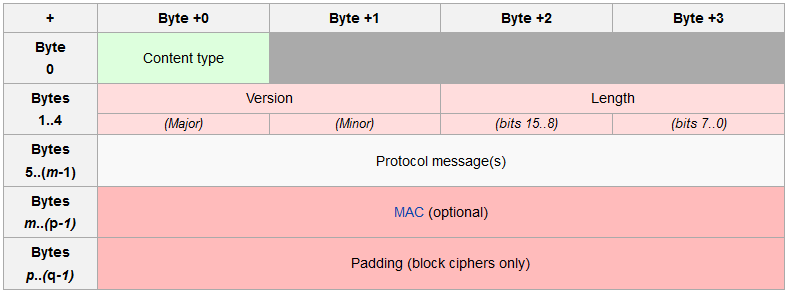
\includegraphics[width=1\textwidth]{diagrams/tls_record.png}\end{figure}

The above figure depicts the general format of all TLS records.

The first field defines the Record Layer Protocol Type of the record, which can
be one of the following:

\begin{table}[H] \centering \begin{tabular}{ | l | l | } \hline \textbf{Hex} &
\textbf{Type} \\ \hline 0x14 & ChangeCipherSpec \\ 0x15 & Alert \\ 0x16 &
Handshake \\ 0x17 & Application \\ 0x18 & Heartbeat \\ \hline \end{tabular}
\end{table}

The second field defines the TLS version for the record message, which is
identified by the major and minor numbers:

\begin{table}[H] \centering \begin{tabular}{ | l | l | l | } \hline
\textbf{Major} & \textbf{Minor} & \textbf{Version} \\ \hline 3 & 0 & SSL 3.0 \\
3 & 1 & TLS 1.0 \\ 3 & 2 & TLS 1.1 \\ 3 & 3 & TLS 1.2 \\ \hline \end{tabular}
\end{table}

The aggregated length of the payload of the record, the MAC and the padding is
then calculated by the following two fields: \begin{math}256*(bits 15..8) +
(bits 7..0)\end{math}.

Finally, the payload of the record, which, depending on the type, may be
encrypted, the MAC, if provided, and the padding, if needed, make up the rest of
the TLS record.

\section{Man-in-the-Middle}\label{sec:mitm}

A man-in-the-middle attack\footnote{\url{https://en.wikipedia.org/wiki/Man-in-the-middle_attack}}
is a type of cyberattack where a malicious actor inserts themselves into a conversation
between two parties, impersonates both and gains access to information that they were
trying to send to each other. A man-in-the-middle attack allows a malicious actor 
to intercept, send and receive data meant for someone else, or not meant to be sent at all, 
without either outside party knowing until it is too late. 

\begin{figure}[H] \caption{Man-in-the-Middle} \centering
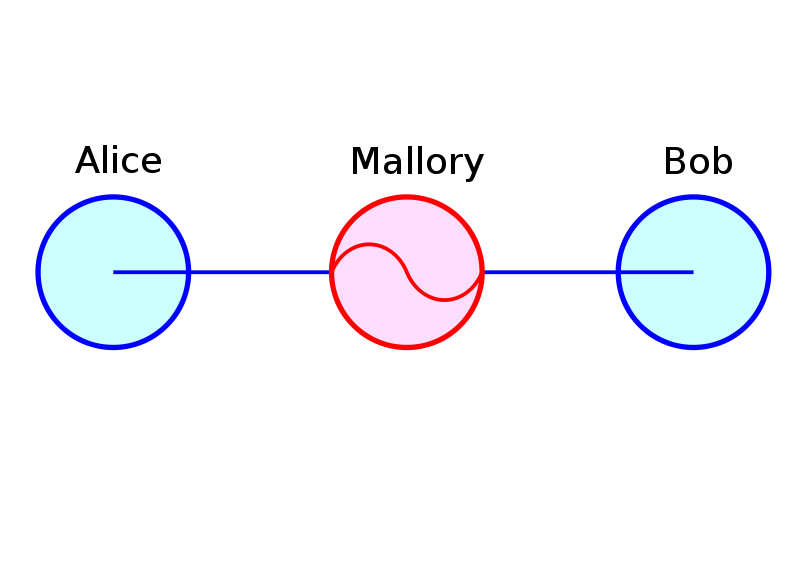
\includegraphics[width=1\textwidth]{diagrams/mitm.png}\end{figure}


MitM attacks can be mitigated using end-to-end encryption, mutual authentication
or PKIs. However, some attacks are still feasible against poorly configured
end-points. Below we describe one such attack, ARP Spoofing.


\subsection{ARP Spoofing}

ARP spoofing\cite{arpspoofing} is a type of attack in which an attacker sends falsified ARP
(Address Resolution Protocol)\cite{arp} messages over a local area network.
This results in the linking of an attacker’s MAC address with the IP address
of a legitimate computer or server on the network. This enables the attacker to
begin receiving any data that is intended for that IP address. ARP spoofing can 
enable malicious parties to intercept, modify or even stop data in-transit.

ARP spoofing can also be used for legitimate reasons, when a developer needs to
debug IP traffic between two hosts. The developer can then act as proxy between
the two hosts, configuring a switch that is used by the two parties to forward
the traffic to the proxy for monitoring purposes.

\begin{figure}[H] \caption{ARP Spoofing} \centering
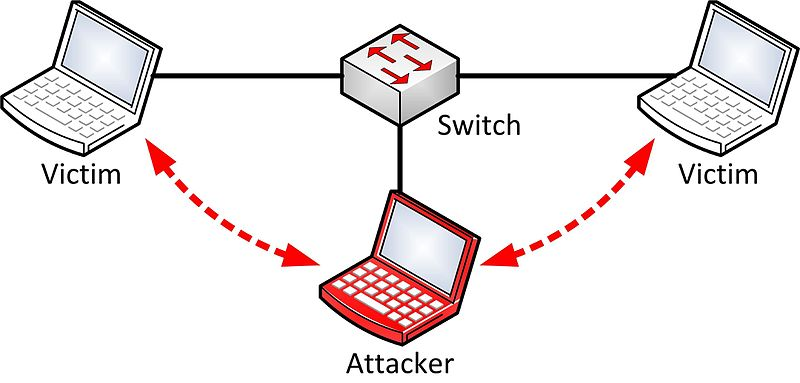
\includegraphics[width=0.8\textwidth]{diagrams/arp_spoofing.jpg}\end{figure}


